\documentclass[10pt,a4paper]{article}
\usepackage[utf8]{inputenc}
\usepackage[german]{babel}
\usepackage{amsmath}
\usepackage{amsfonts}
\usepackage{amssymb}
\usepackage{graphicx}
\usepackage{float}
\usepackage[left=2cm,right=2cm,top=2cm,bottom=2cm]{geometry}

\begin{document}

\section*{Aufgabe 9.2}

Das Diagramm ist nicht korrekt gezeichnet.
Das a müsste über den mittleren Spalten stehen.
So wie es im Moment ist, kann das Diagramm keinen Fall $(ac)$ abbilden, sondern nur $(\overline{a}c)$ und $(a\overline{c})$.

Ein zweiter Fehler ist, dass die beiden oberen, rechten Felder $1$ sein müssten, weil der Ausdruck immer wahr ist für $(\overline{b}c)$.

\section*{Aufgabe 9.3}

\subsection*{Teil 1}

\begin{equation}
\overline{a}\overline{b}\overline{c} + \overline{a}b\overline{c} + \overline{a}bc + ab\overline{c} + abc
\end{equation}

\subsection*{Teil 2}

\begin{equation}
(a + b + \overline{c})(\overline{a} + b + c)(\overline{a} + b + \overline{c})
\end{equation}

\subsection*{Teil 3 + 4}

\begin{figure}[H]
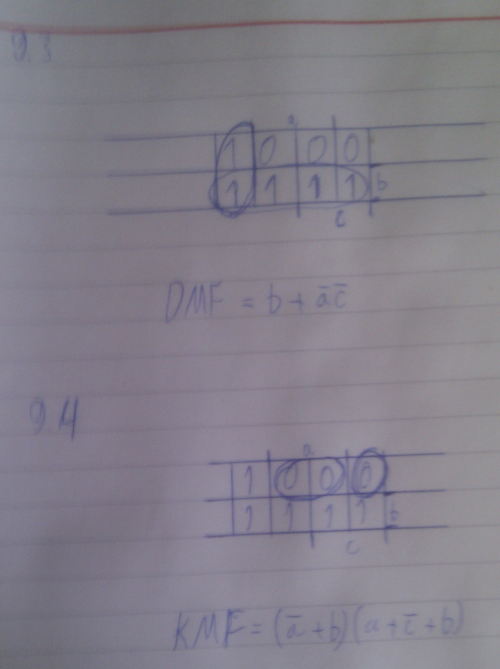
\includegraphics[width=400pt]{9_3,4}
\end{figure}

Die KMF ist doch $(\overline{a} + b)(b + \overline{c})$, entgegen dem, was ich im Bild geschrieben habe.

\subsection*{Teil 5}

\begin{align*}
\overline{a}\overline{b}\overline{c} + \overline{a}b\overline{c} + \overline{a}bc + ab\overline{c} + abc & = \overline{a}(\overline{b}\overline{c} + b\overline{c} + bc) + ab(\overline{c} + c)\\
& = \overline{a}(\overline{b}\overline{c} + b(\overline{c} + c)) + ab\\
& = \overline{a}(\overline{b}\overline{c} + b) + ab\\
& = \overline{a}\overline{b}\overline{c} + \overline{a}b + ab\\
& = \overline{a}\overline{b}\overline{c} + (\overline{a} + a)b\\
& = (\overline{a} + b)(\overline{b} + b)(\overline{c} + b)\\
& = (\overline{a} + b)(\overline{c} + b)\\
& = b + \overline{a}\overline{c}
\end{align*}

\begin{align*}
(a + b + \overline{c})(\overline{a} + b + c)(\overline{a} + b + \overline{c}) & = ((a + b + \overline{c})\overline{a} + (a + b + \overline{c})b + (a + b + \overline{c})c)(\overline{a} + b + \overline{c})\\
& = ((a\overline{a} + b\overline{a} + \overline{c}\overline{a}) + (ab + bb + \overline{c}b) + (ac + bc + \overline{c}c)c)(\overline{a} + b + \overline{c})\\
& = ((b\overline{a} + \overline{c}\overline{a}) + (ab + b + \overline{c}b) + (ac + bc))(\overline{a} + b + \overline{c})\\
& = (b\overline{a} + \overline{c}\overline{a} + ab + b + \overline{c}b + ac + bc)(\overline{a} + b + \overline{c})\\
& = (b\overline{a} + ab + \overline{c}b + bc + b + \overline{c}\overline{a} + ac)(\overline{a} + b + \overline{c})\\
& = (b(\overline{a} + a + \overline{c} + c + 1) + \overline{c}\overline{a} + ac)(\overline{a} + b + \overline{c})\\
& = (b + \overline{c}\overline{a} + ac)(\overline{a} + b + \overline{c})\\
& = ((b + \overline{c}\overline{a} + ac)\overline{a} + (b + \overline{c}\overline{a} + ac)b + (b + \overline{c}\overline{a} + ac)\overline{c})\\
& = ((b\overline{a} + \overline{c}\overline{a}\overline{a} + ac\overline{a}) + (bb + \overline{c}\overline{a}b + acb) + (b\overline{c} + \overline{c}\overline{a}\overline{c} + ac\overline{c}))\\
& = (b\overline{a} + \overline{c}\overline{a}\overline{a} + ac\overline{a} + bb + \overline{c}\overline{a}b + acb + b\overline{c} + \overline{c}\overline{a}\overline{c} + ac\overline{c})\\
& = (b\overline{a} + \overline{c}\overline{a} + b + \overline{c}\overline{a}b + acb + b\overline{c} + \overline{c}\overline{a} + ac\overline{c})\\
& = (b\overline{a} + b + \overline{c}\overline{a}b + acb + b\overline{c} + \overline{c}\overline{a} + \overline{c}\overline{a} + ac\overline{c})\\
& = b(\overline{a} + 1 + \overline{c}\overline{a} + ac + \overline{c}) + \overline{c}(\overline{a} + \overline{a} + ac)\\
& = b + \overline{c}(\overline{a} + ac)\\
& = b + (\overline{a}\overline{c} + ac\overline{c})\\
& = b + \overline{a}\overline{c}
\end{align*}

\begin{equation}
b + \overline{a}\overline{c} = (b + \overline{a})(b + \overline{c}) = (\overline{a} + b)(\overline{c} + b)
\end{equation}

\subsection*{Teil 6}

Unter diesen Bedingungen kostet jede $NOT$-Operation $1$ und jeden $AND$- und $OR$-Operation $1$ für jeden Operanden.
Somit ergibt sich
\begin{equation}
Kosten(DMF) = 6
\end{equation}
\begin{equation}
Kosten(KMF) = 9
\end{equation}

\subsection*{Teil 7}

\begin{equation}
DMF = b + \overline{a}\overline{c}
\end{equation}
\begin{figure}[H]
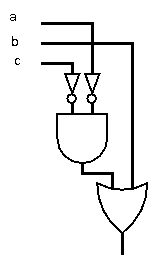
\includegraphics[width=150pt]{9_7}
\end{figure}

\subsection*{Teil 8}

\begin{equation}
b + \overline{a}\overline{c} = \overline{\overline{b + \overline{(\overline{a + a}) + (\overline{c + c})}} + \overline{b + \overline{(\overline{a + a}) + (\overline{c + c})}}}
\end{equation}
\begin{figure}[H]
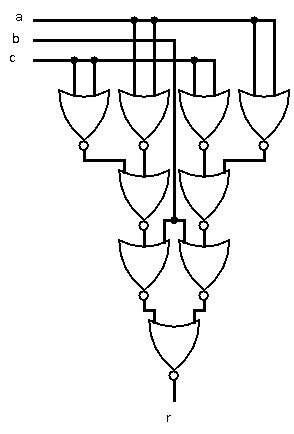
\includegraphics[width=200pt]{9_8}
\end{figure}

\end{document}